\documentclass{article}
\usepackage{listings}
\usepackage{booktabs}
\usepackage{here}
\usepackage{subcaption}
\usepackage{tikz}
\usepackage{amsmath}
\usepackage{graphicx}
\usepackage[colorlinks=true, allcolors=black]{hyperref}

% Set page size and margins
\usepackage[letterpaper,top=2cm,bottom=2cm,left=3cm,right=3cm,marginparwidth=1.75cm]{geometry}

% % Remove section numbering
% \renewcommand{\thesection}{}
% \renewcommand{\thesubsection}{}

% \newcommand{\code}[1]{{\tt #1}}
% \newcommand\blankpage{%
% 	\null
% 	\thispagestyle{empty}%
% 	\addtocounter{page}{-1}%
% 	\newpage}


%%%% Define style for code %%%%
\lstdefinestyle{mystyle}{
    language=Java,
	numbers=left,
    basicstyle=\ttfamily\footnotesize,
    keywordstyle=\color{blue},
    commentstyle=\color{gray},
    stringstyle=\color{brown},
    showstringspaces=false,
    breaklines=true,
    frame=single, % Aggiunge il bordo
    frameround=tttt, % Angoli arrotondati
    backgroundcolor=\color{lightgray!20}, % Sfondo leggermente grigio
    rulecolor=\color{black}, % Colore del bordo
}
\lstset{style=mystyle} % stile definito come default
\captionsetup[lstlisting]{labelformat=empty} % Disable listing numbering
%%%%%%%%%%%%%%%%%%%%%%%%%%%%%%

\newcommand{\codepath}{../app/src/main/java/com/example/stepappv4}


\title{
	\normalfont\normalsize
	\textsc{Mobile and Wearable Computing SA 2024-2025\\%
	Universit\`a della Svizzera italiana}\\
	\vspace{25pt}
	\rule{\linewidth}{0.5pt}\\
	\vspace{20pt}
	{\huge Assignment 2}\\
	\vspace{12pt}
	\rule{\linewidth}{1pt}\\
	\vspace{12pt}
}

\author{
  Paolo Deidda \\
  \text{paolo.deidda@usi.ch} \\ 
  \url{https://github.com/USI-Projects-Collection/MWCTutorial04.git}
}


\begin{document}
\maketitle

\tableofcontents

\vspace{2cm}

\section*{Important notes}
Please note that when testing in \texttt{Android Studio}'s emulator the \texttt{TYPE\_STEP\_DETECTOR} sensor probably won't respond. However the application works fine when installed on a real \texttt{Android} Phone. \\

If you want to test the rest of the exercises on the emulator simply switch the sensor. Uncomment \texttt{TYPE\_LINEAR\_ACCELERATOR} (\textit{line 63}) and comment \textit{line 64}.

\lstinputlisting[
    firstline=63, 
    lastline=64, 
    firstnumber=63,
    caption=\texttt{\codepath/ui/steps/StepsFragment.java}
]{\codepath/ui/steps/StepsFragment.java}

\newpage
\section{Data storage and visualization}
    
    As can be seen in Figure~\ref{fig:thePicture} the Report fragment has now a two switch tab
    that allows the user to select the time chunks for the chart in the same View.
    
\subsection{fragment\_report.xml}\label{subsec:fragment_report.xml}
        The first thing I needed to was to add was the \textbf{TabLayout} in file
        \textit{fragment\_report.xml}.

    \lstinputlisting[
        firstline=10,
        lastline=16,
        firstnumber=10,
        caption=\texttt{\codepath/res/layout/fragment\_report.xml}
        ,label={lst:frag}
    ]{\codepath/res/layout/fragment_report.xml}
    
    I also rename the \textbf{AnyChartView} from \textit{hourBarChart} to \textit{barChart}
        since it will now follow a double purpose not only for hourly display but also for daily
        count of steps.
    
\subsection{StepAppOpenHelper.java}
    


\subsection{ReportFragment.java}






\newpage
\section{Exercise 2 – Material Design}
    
    \subsection{Change App Icon}
        To change our app's icon, I used Android Studio's built-in feature to generate icons (see Figure~\ref{fig:ex2_1.1}). I navigated to the \texttt{res} folder, right-clicked on the \texttt{drawable} folder, and selected \textit{New} $\rightarrow$ \textit{Image Asset}. After selecting the image I had previously imported, Android Studio automatically generated the required icons.
        
        \begin{figure}[H]
            \centering
            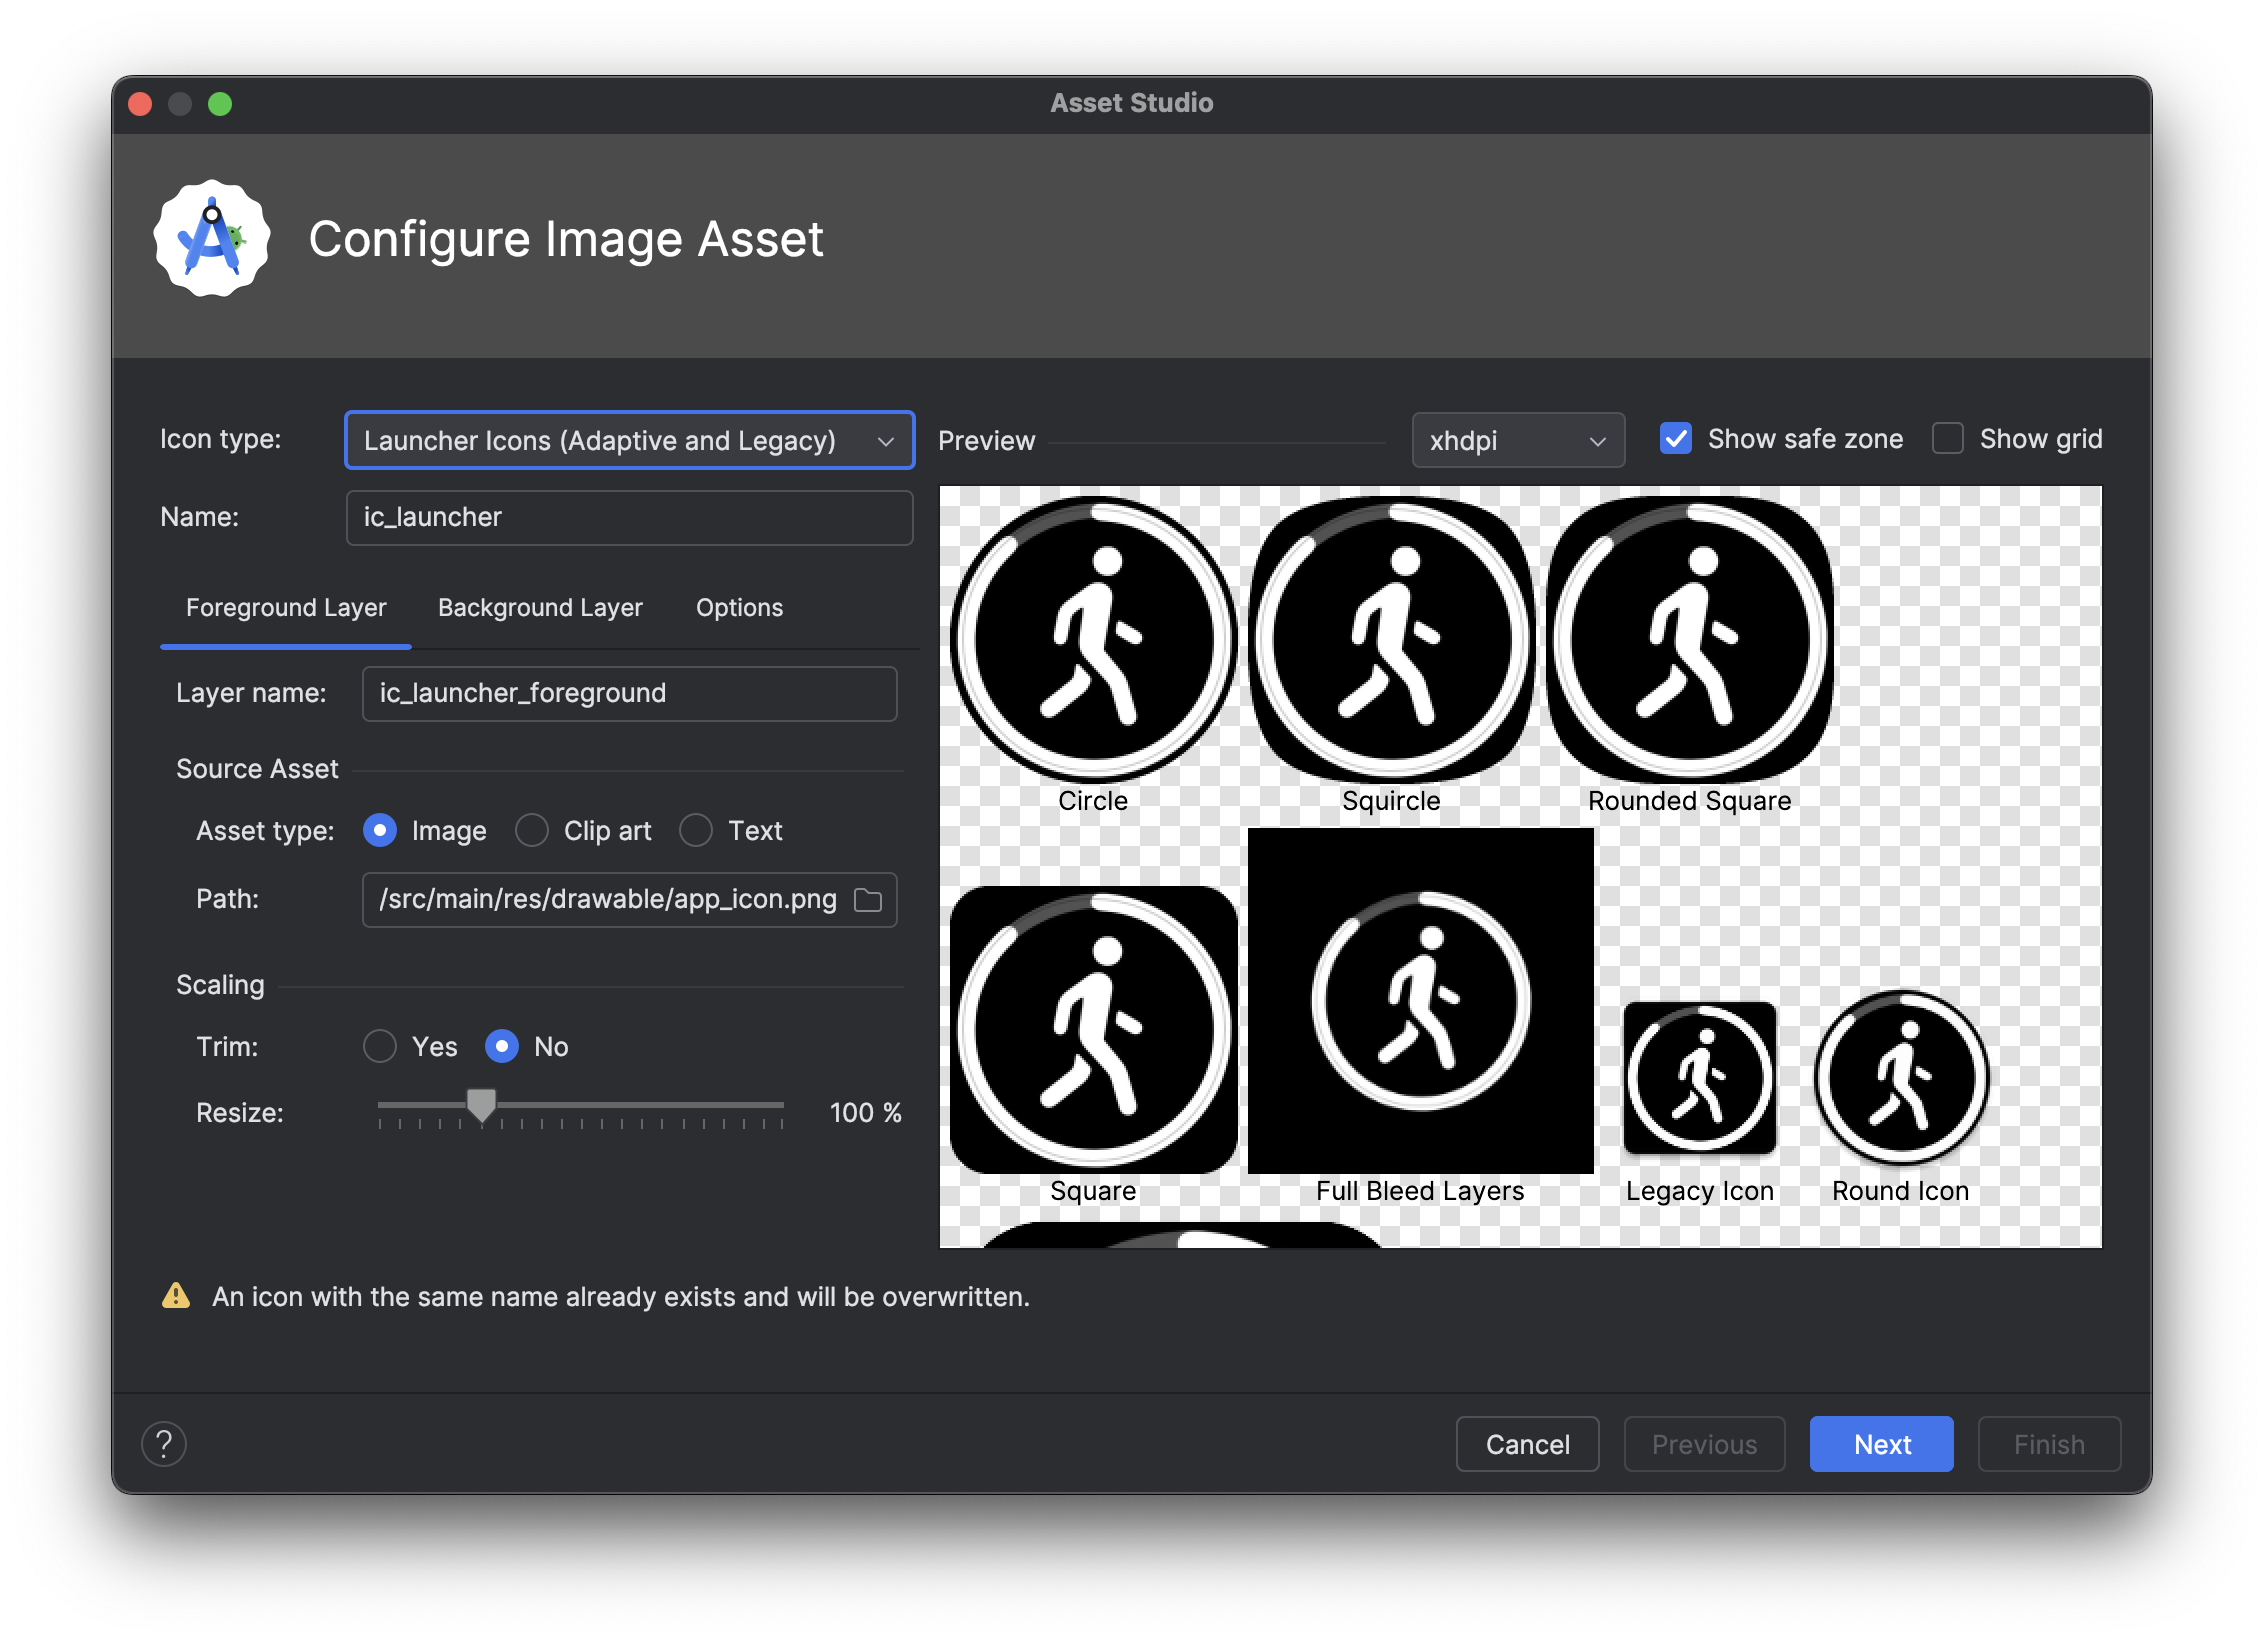
\includegraphics[width=0.5\textwidth]{res/img/appIcon.png}
            \caption{Generating Icons in Android Studio}
            \label{fig:ex2_1.1}
        \end{figure}
        
        Android Studio handled the generation of all necessary formats for the image, including various resolution sizes and shapes (see Figure~\ref{fig:ex2_2.2}).
        
        \begin{figure}[H]
            \centering
            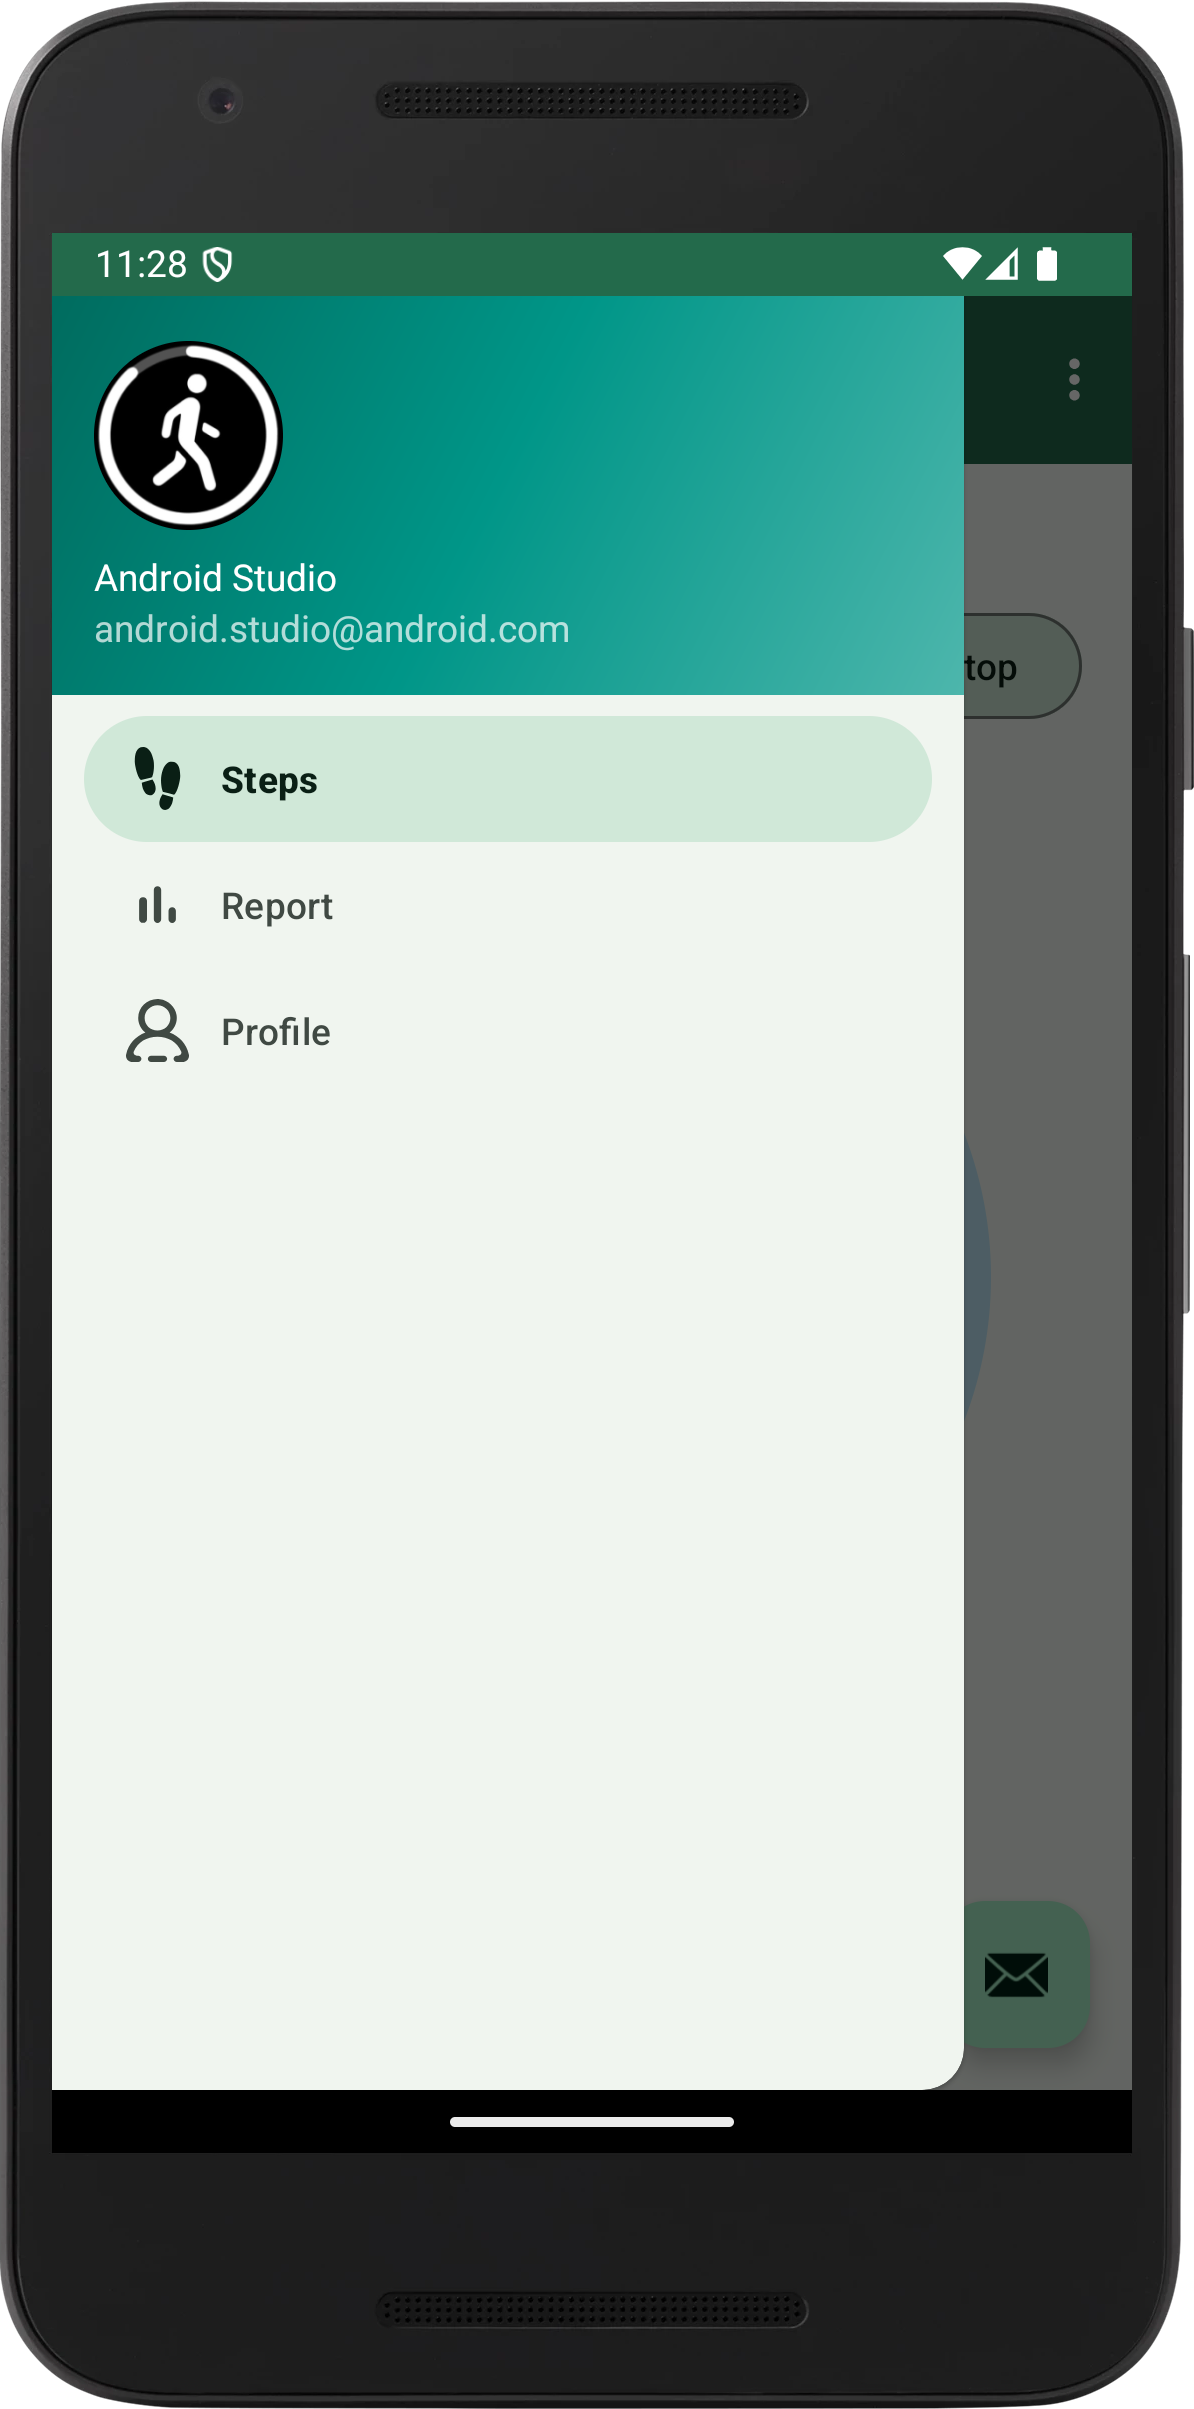
\includegraphics[width=0.20\textwidth]{res/img/icon1.png}
            \hspace{0.05\textwidth}
            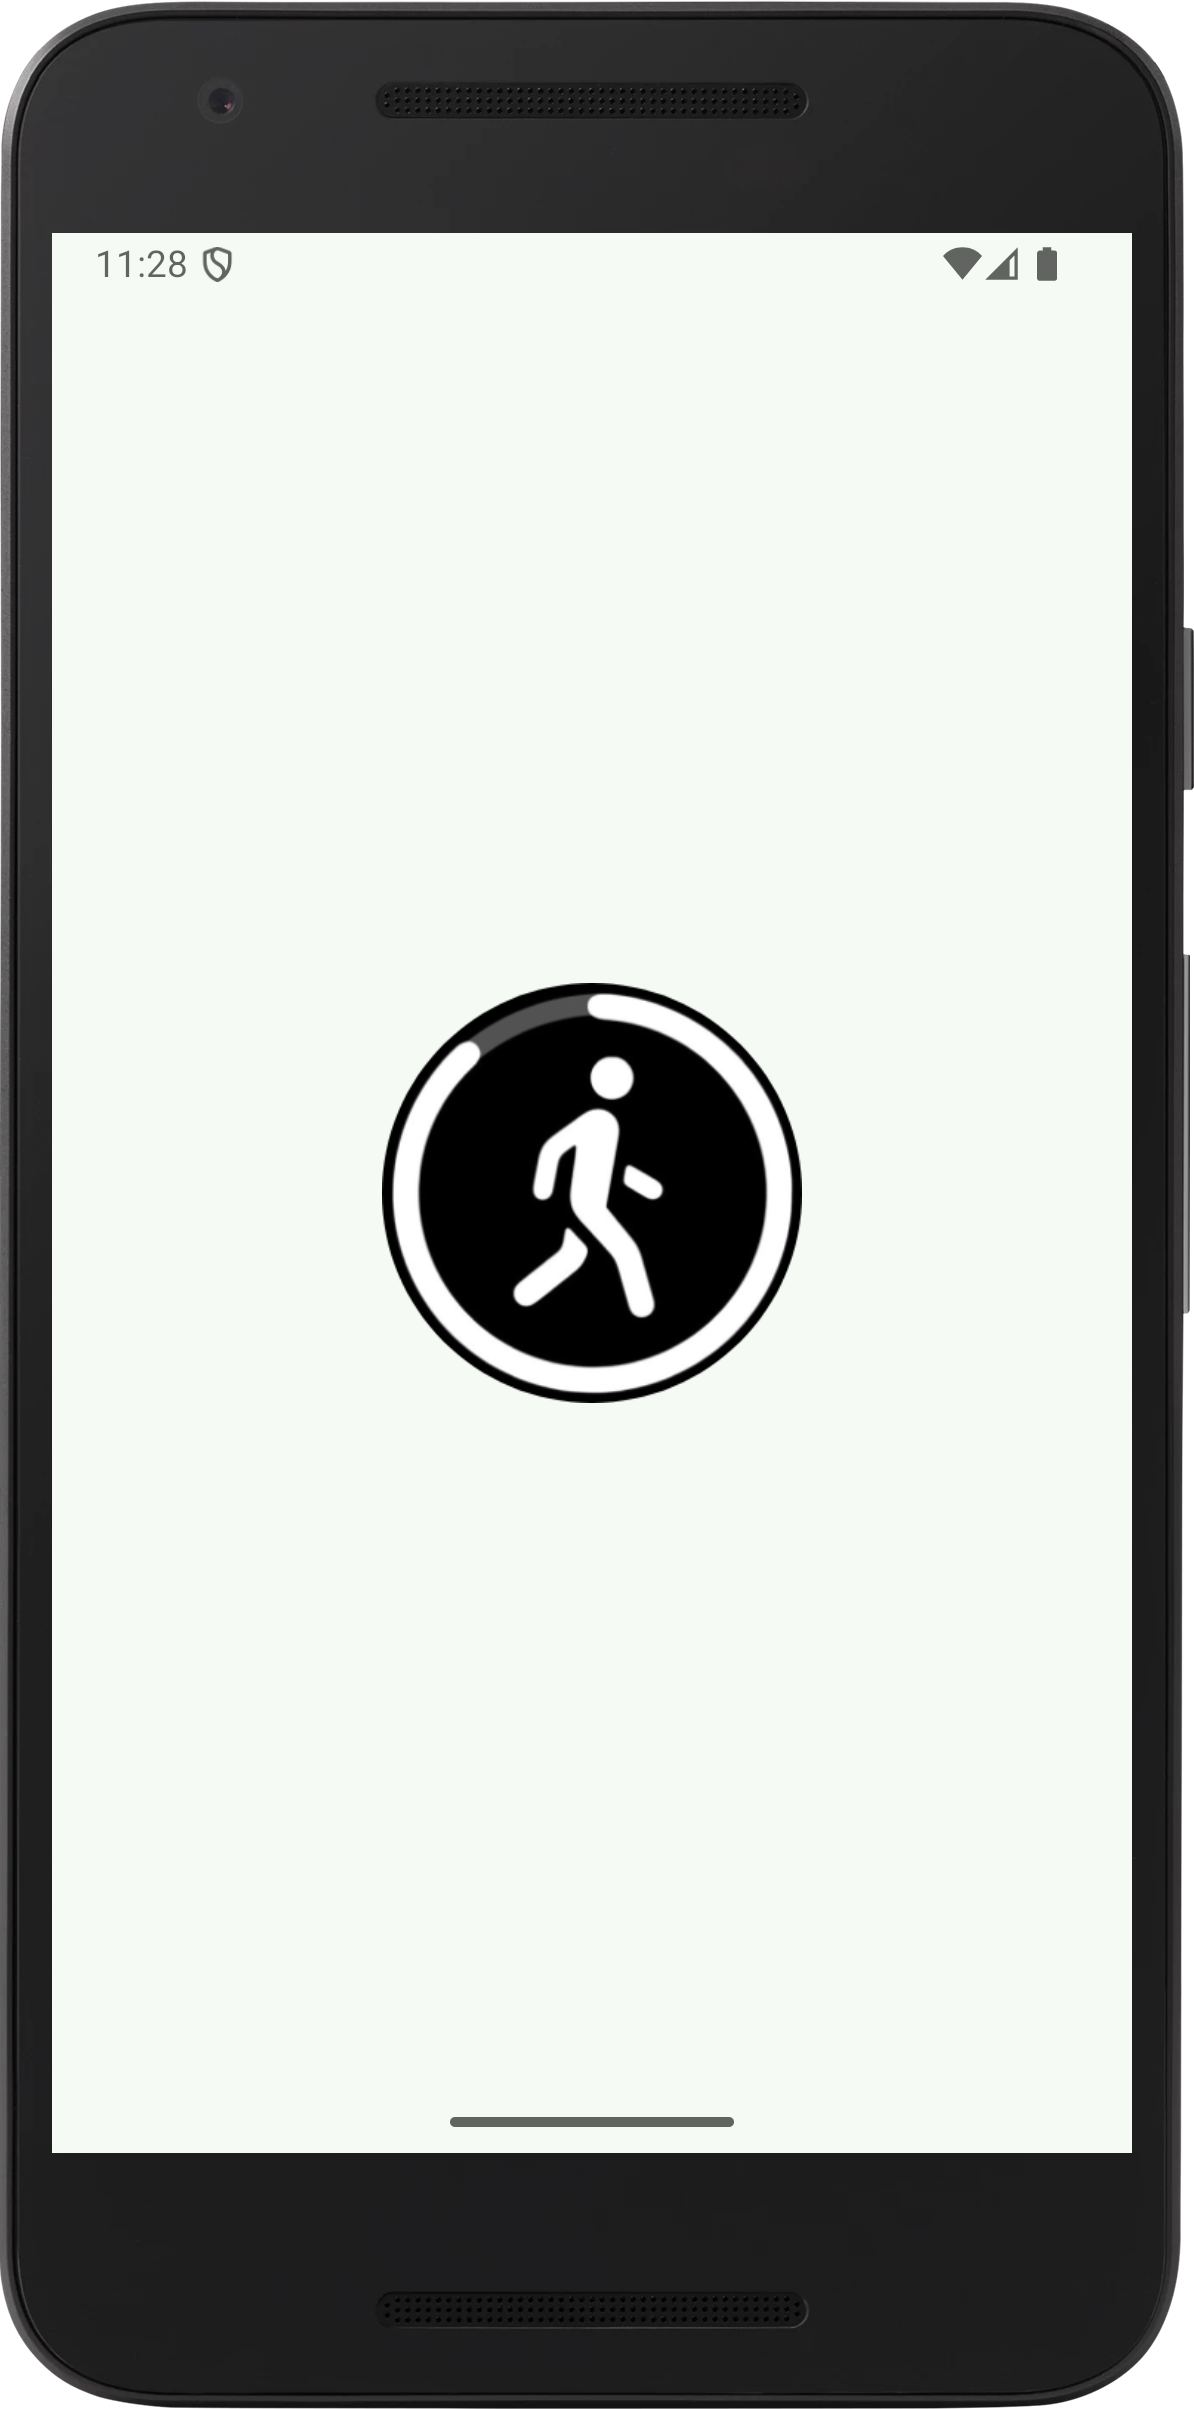
\includegraphics[width=0.20\textwidth]{res/img/icon2.png}      
            \hspace{0.05\textwidth}
            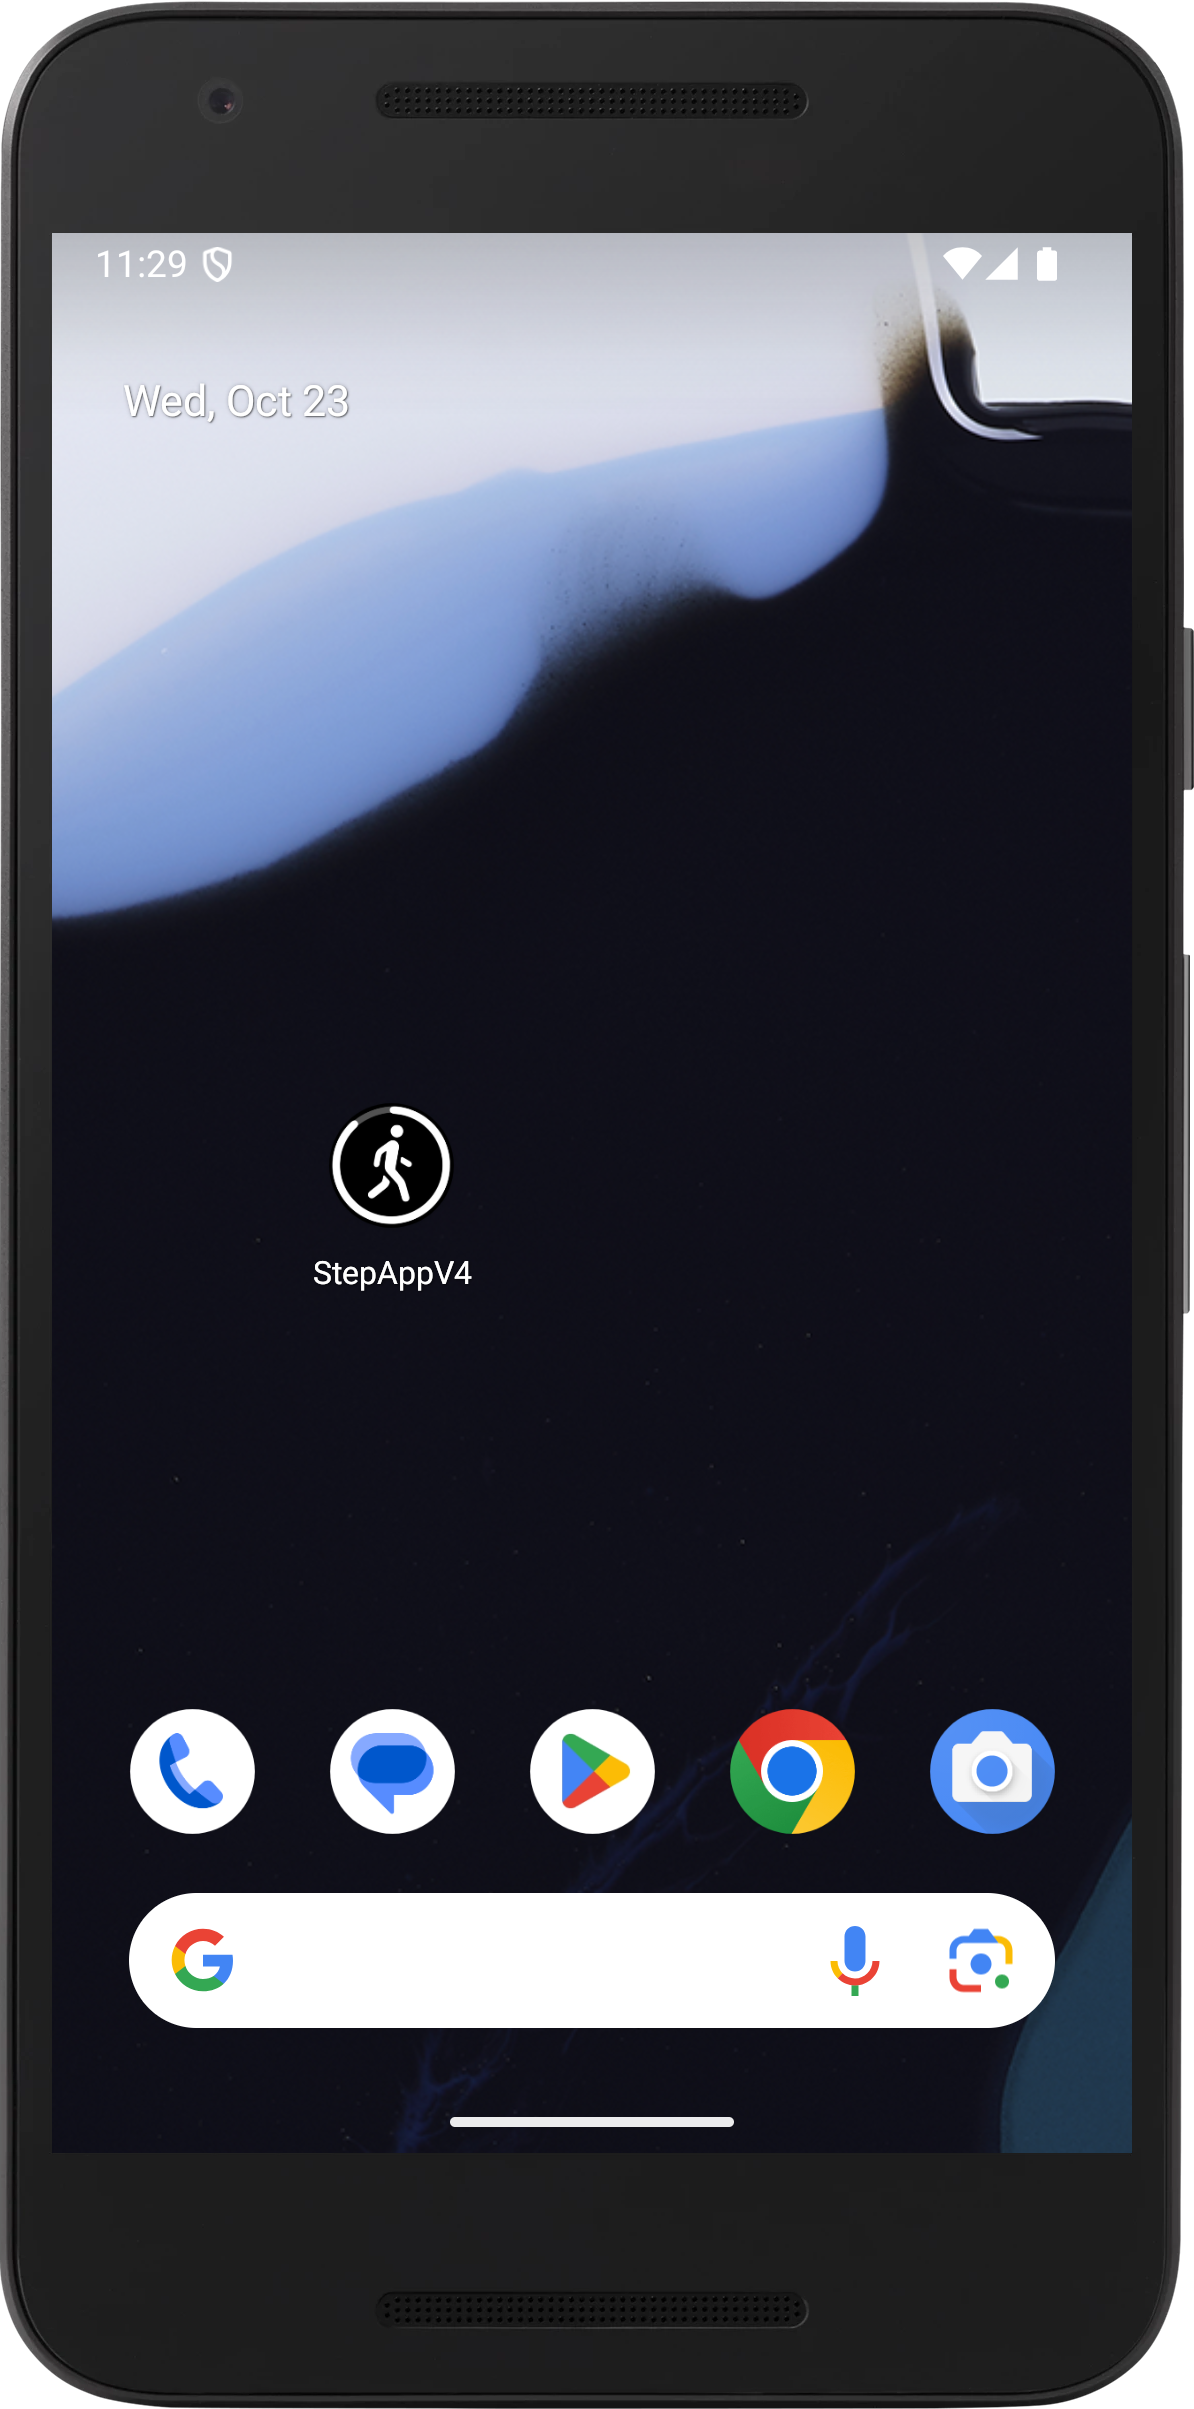
\includegraphics[width=0.20\textwidth]{res/img/icon3.png}
            \caption{Generated Icons with Different Resolutions and Shapes}
            \label{fig:ex2_2.2}
        \end{figure}



\newpage


\subsection{Implement Dark Theme}
    To implement the dark theme, I utilized the \texttt{AppCompatDelegate} class provided by Android's support library. This allows for easy switching between light and dark modes. The dark mode can be toggled by the user via a switch placed in the \texttt{Profile} page (see Figure~\ref{fig:ex2_3}).

    \begin{figure}[H]
        \centering
        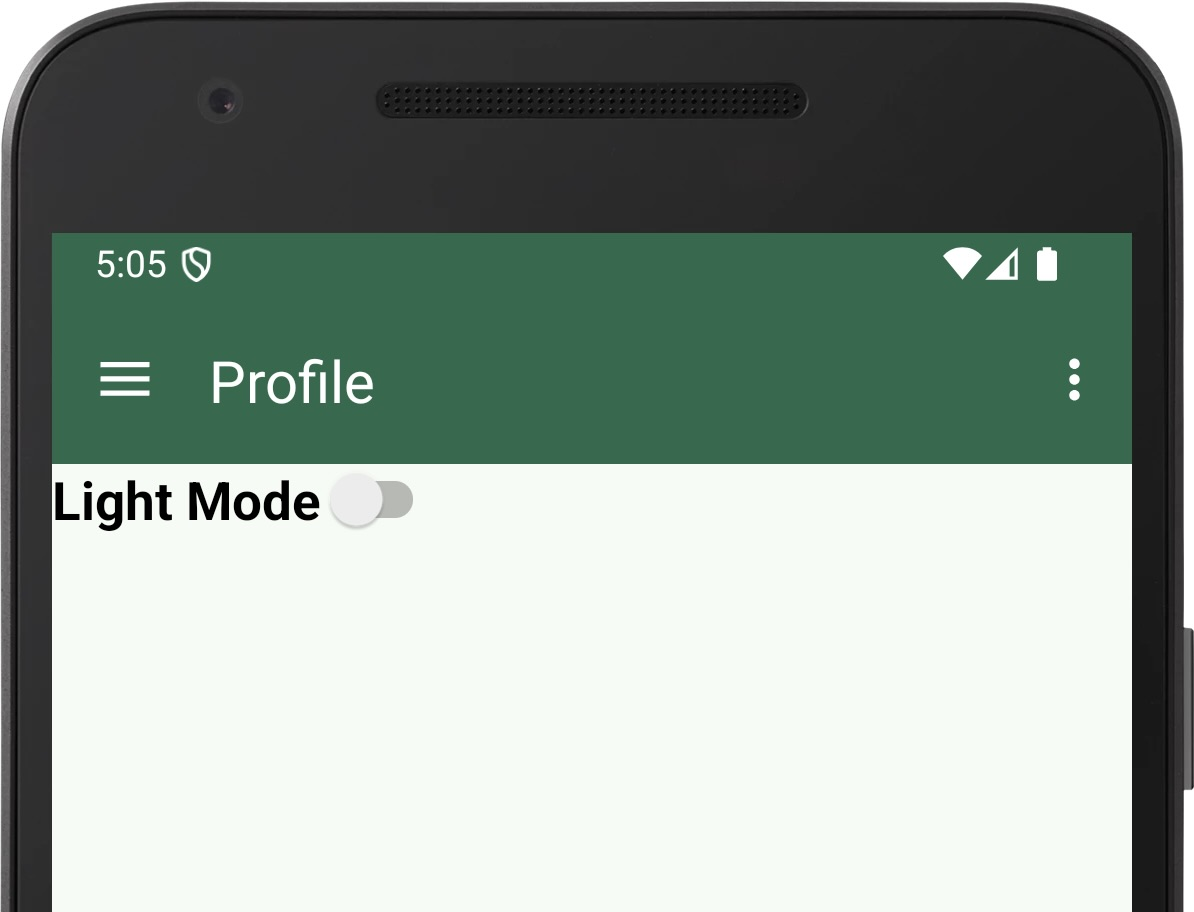
\includegraphics[width=0.30\textwidth]{res/img/dark_theme_switch.png}
        \caption{Switch for toggling between Light and Dark Modes}
        \label{fig:ex2_3}
    \end{figure}

    The dark mode implementation involved modifying the \texttt{ProfileFragment} and adding an \\ \texttt{OnCheckedChangeListener} to the switch. Depending on whether the switch is checked or not, the theme is switched using \texttt{AppCompatDelegate.setDefaultNightMode()}. If the switch is turned on, the dark theme is enabled using \texttt{AppCompatDelegate.MODE\_NIGHT\_YES}, and if the switch is off, the light theme is restored using \texttt{AppCompatDelegate.MODE\_NIGHT\_NO}.

    The relevant code for the theme switching logic is shown below:

    \lstinputlisting[
        firstline=45, 
        lastline=56, 
        firstnumber=45,
        caption=\texttt{\codepath/ui/slideshow/ProfileFragment.java}
    ]{\codepath/ui/slideshow/ProfileFragment.java}

    Additionally, I ensured that the \texttt{colors.xml} file contained separate color definitions for both light and dark modes . This file is located in the \texttt{res/values} and \texttt{res/values-night} directories for light and dark modes, respectively. Same thing I had to do for the Themes, this prevented the app from changing layout changes. The following figures are some screenshots of the app in dark mode (see Figure~\ref{fig:ex2_2.4}).

    \begin{figure}[H]
        \centering
        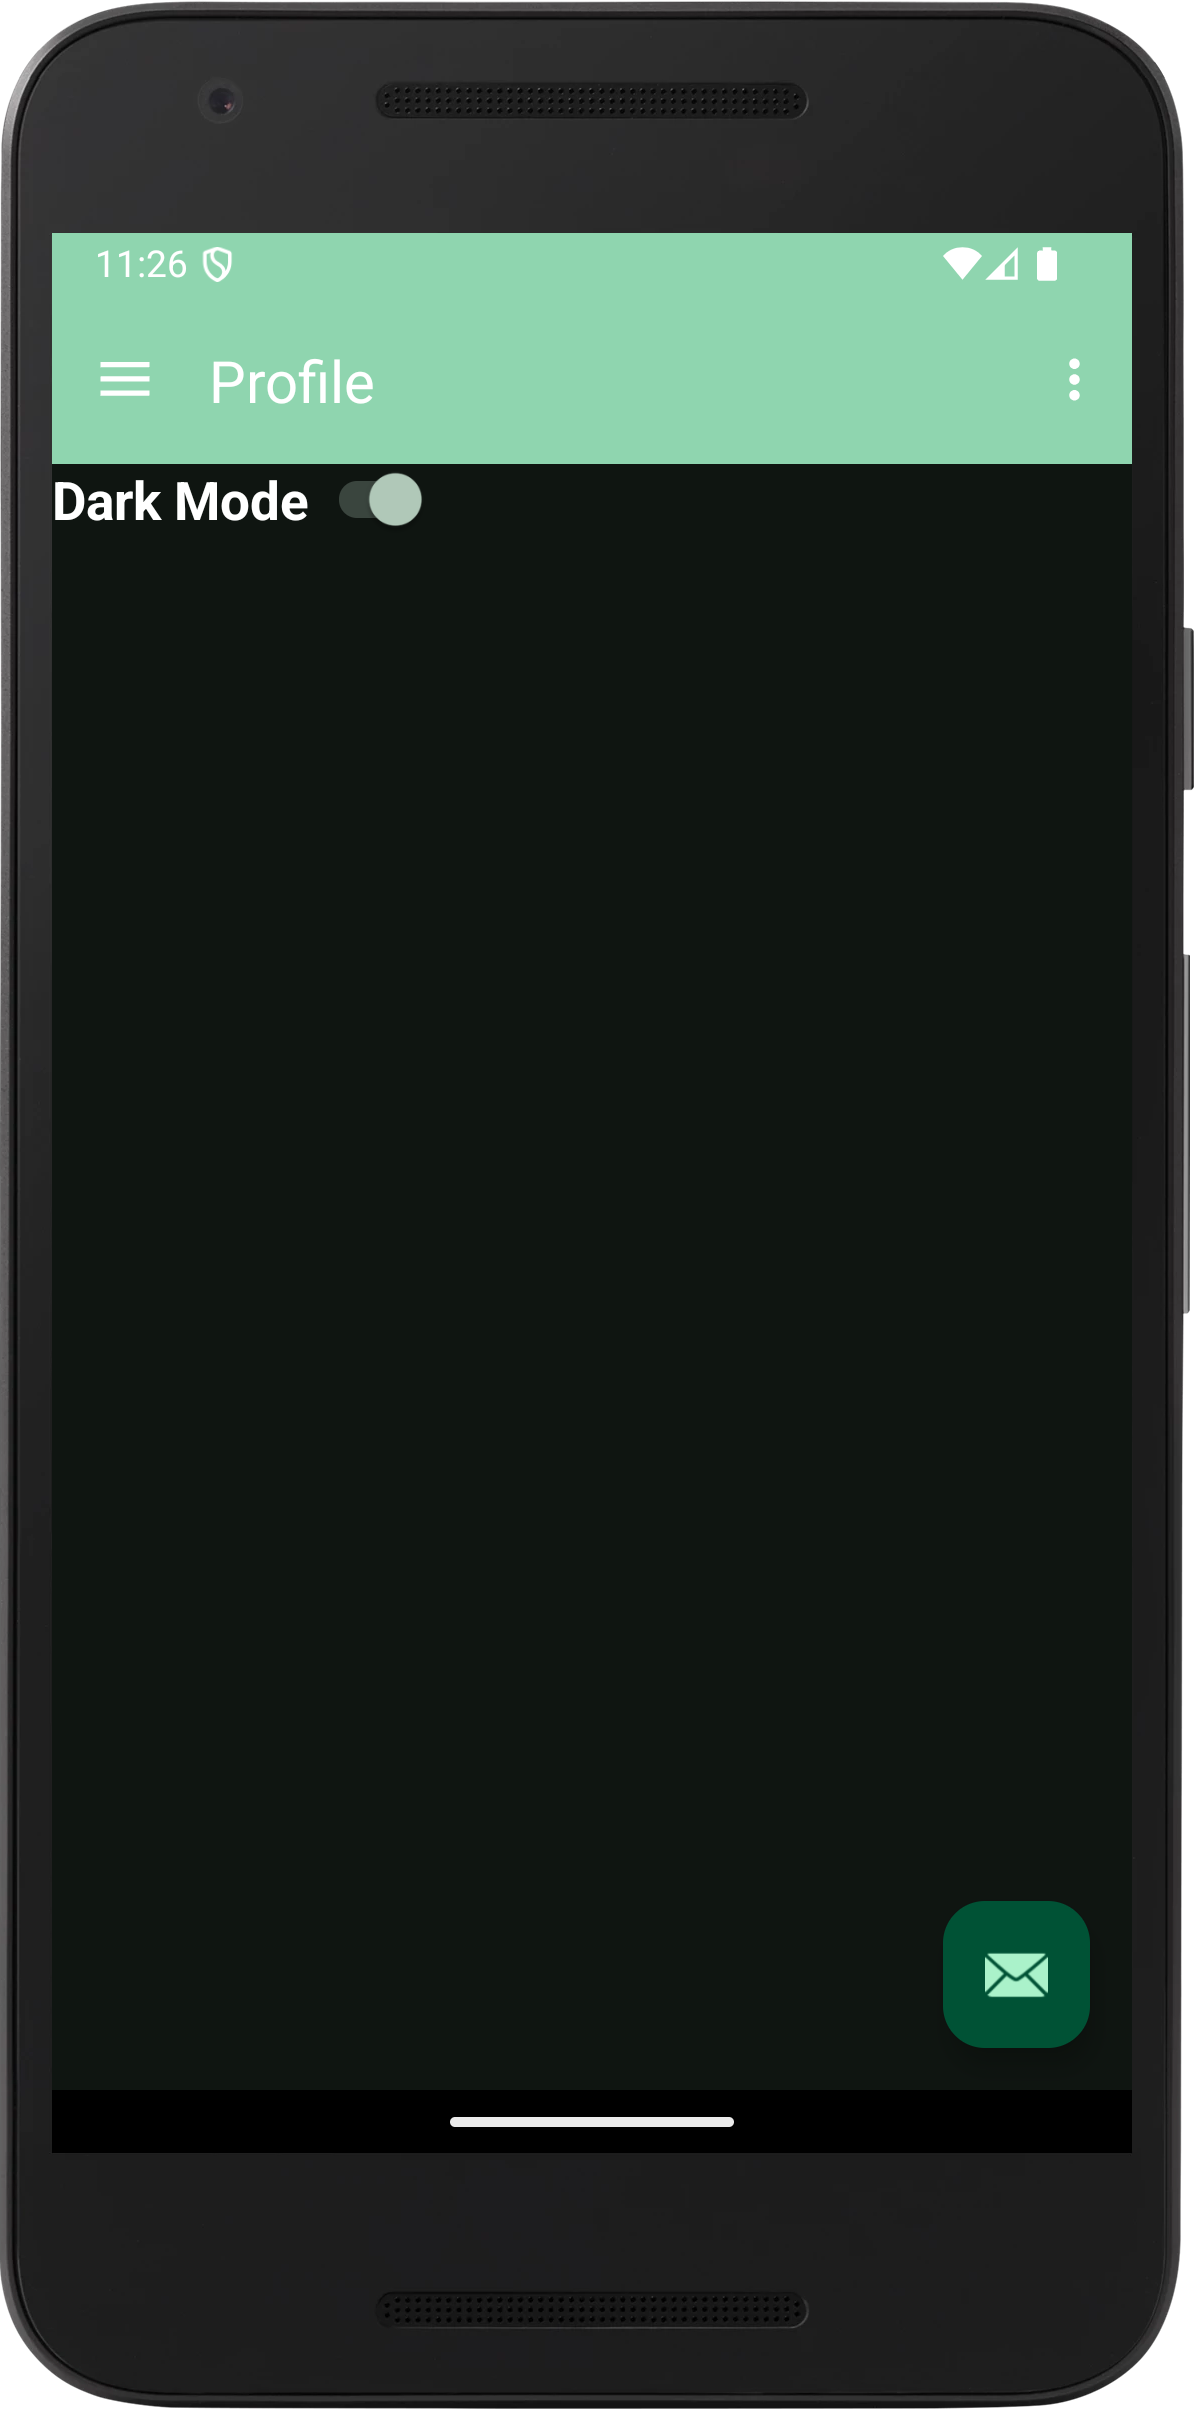
\includegraphics[width=0.15\textwidth]{res/img/darkMode1.png}
        \hspace{0.05\textwidth}
        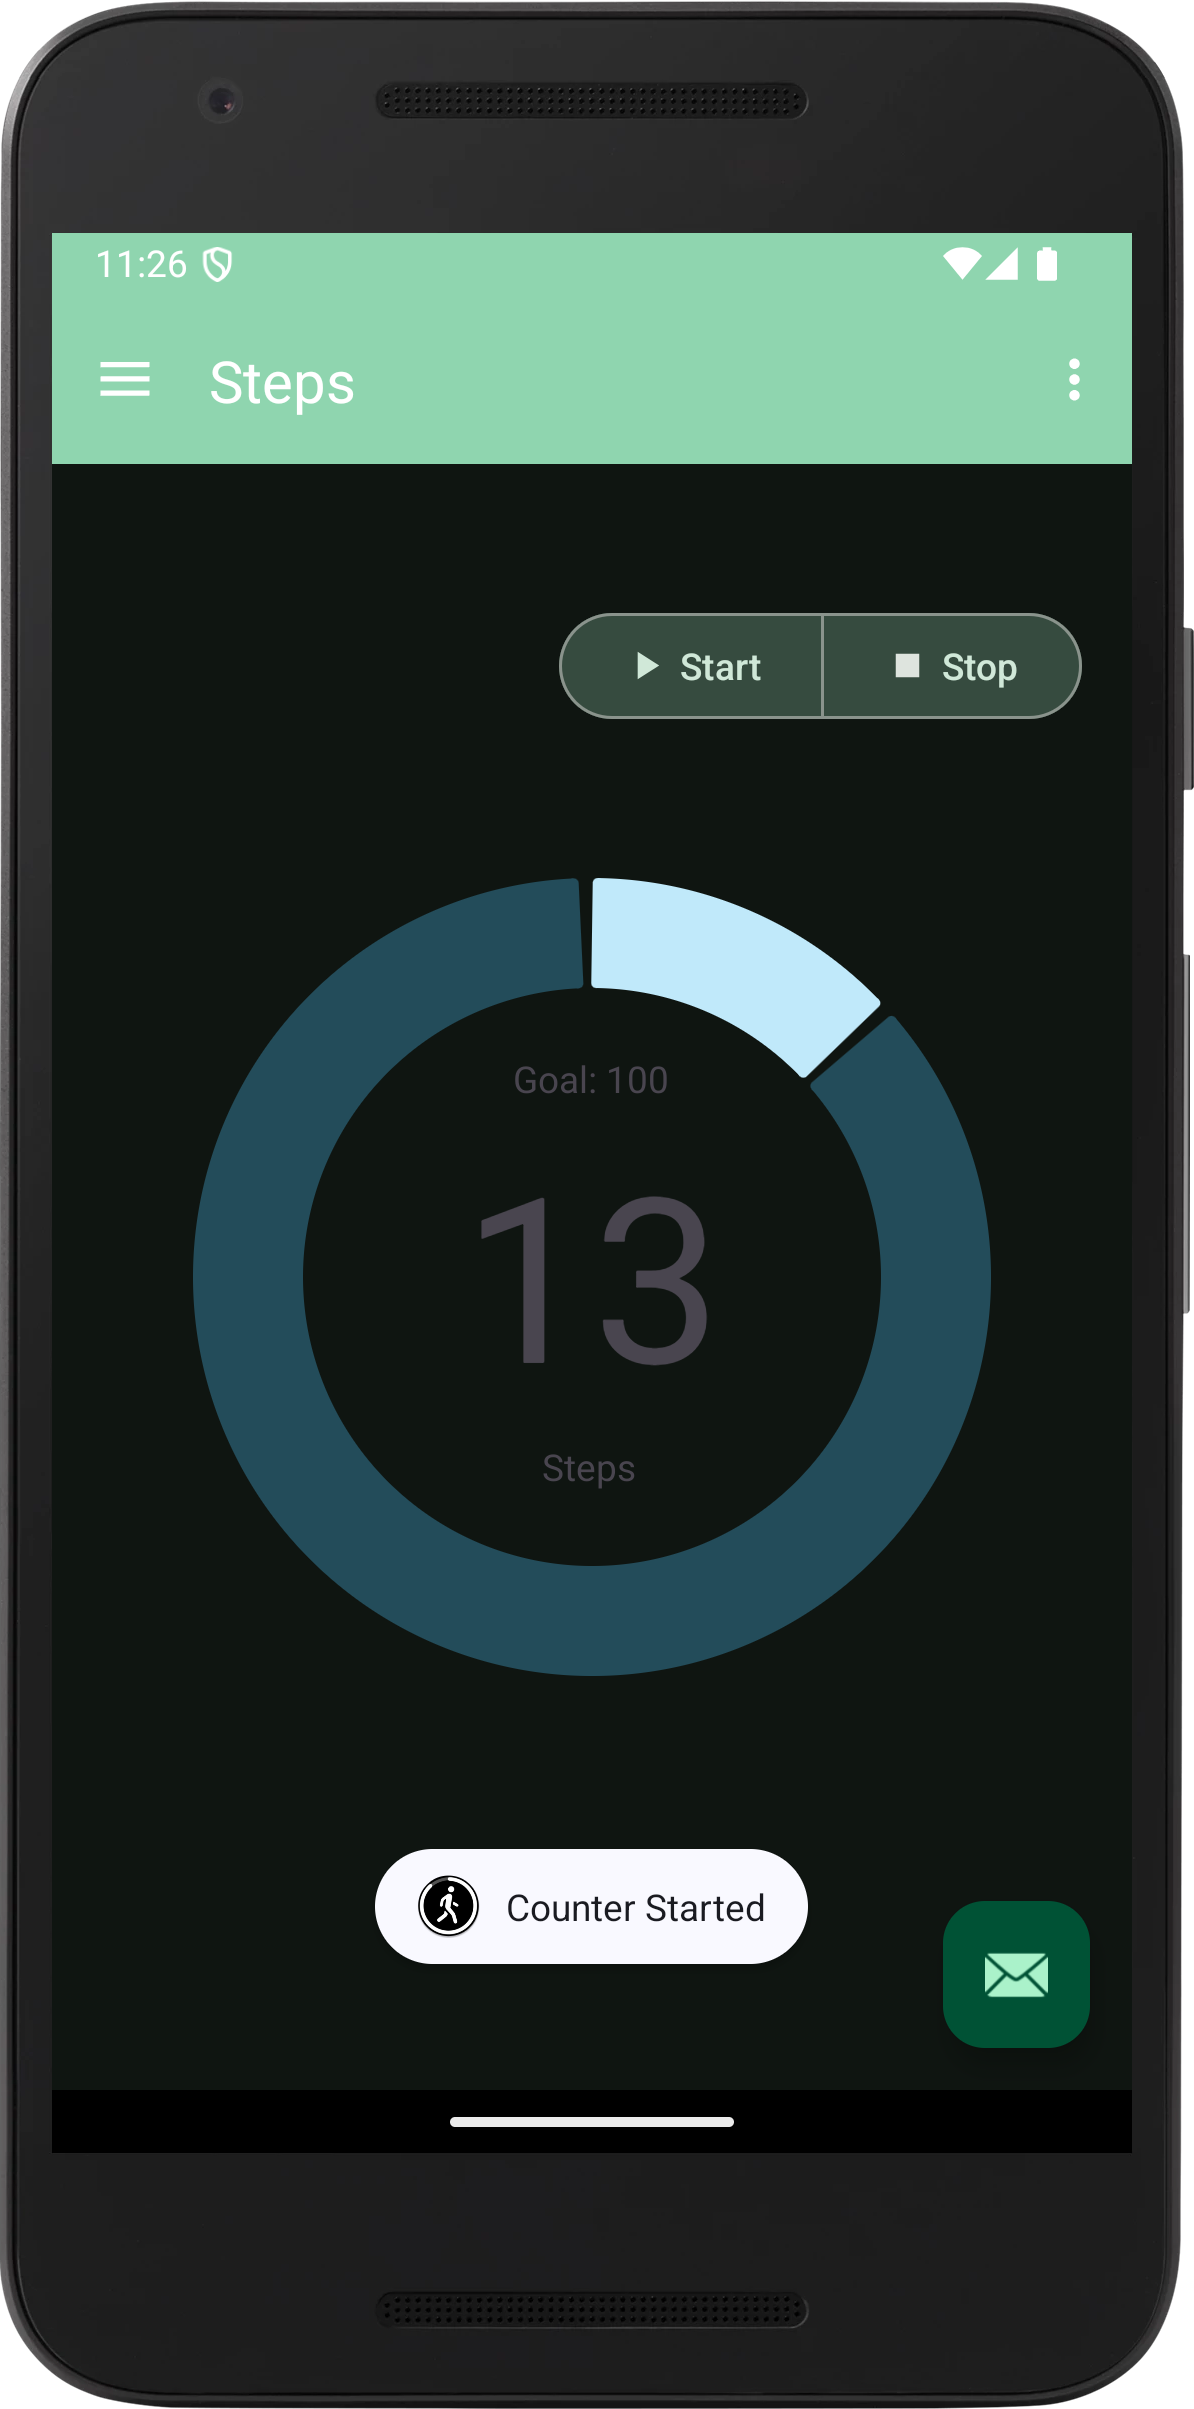
\includegraphics[width=0.15\textwidth]{res/img/darkMode2.png}      
        \hspace{0.05\textwidth}
        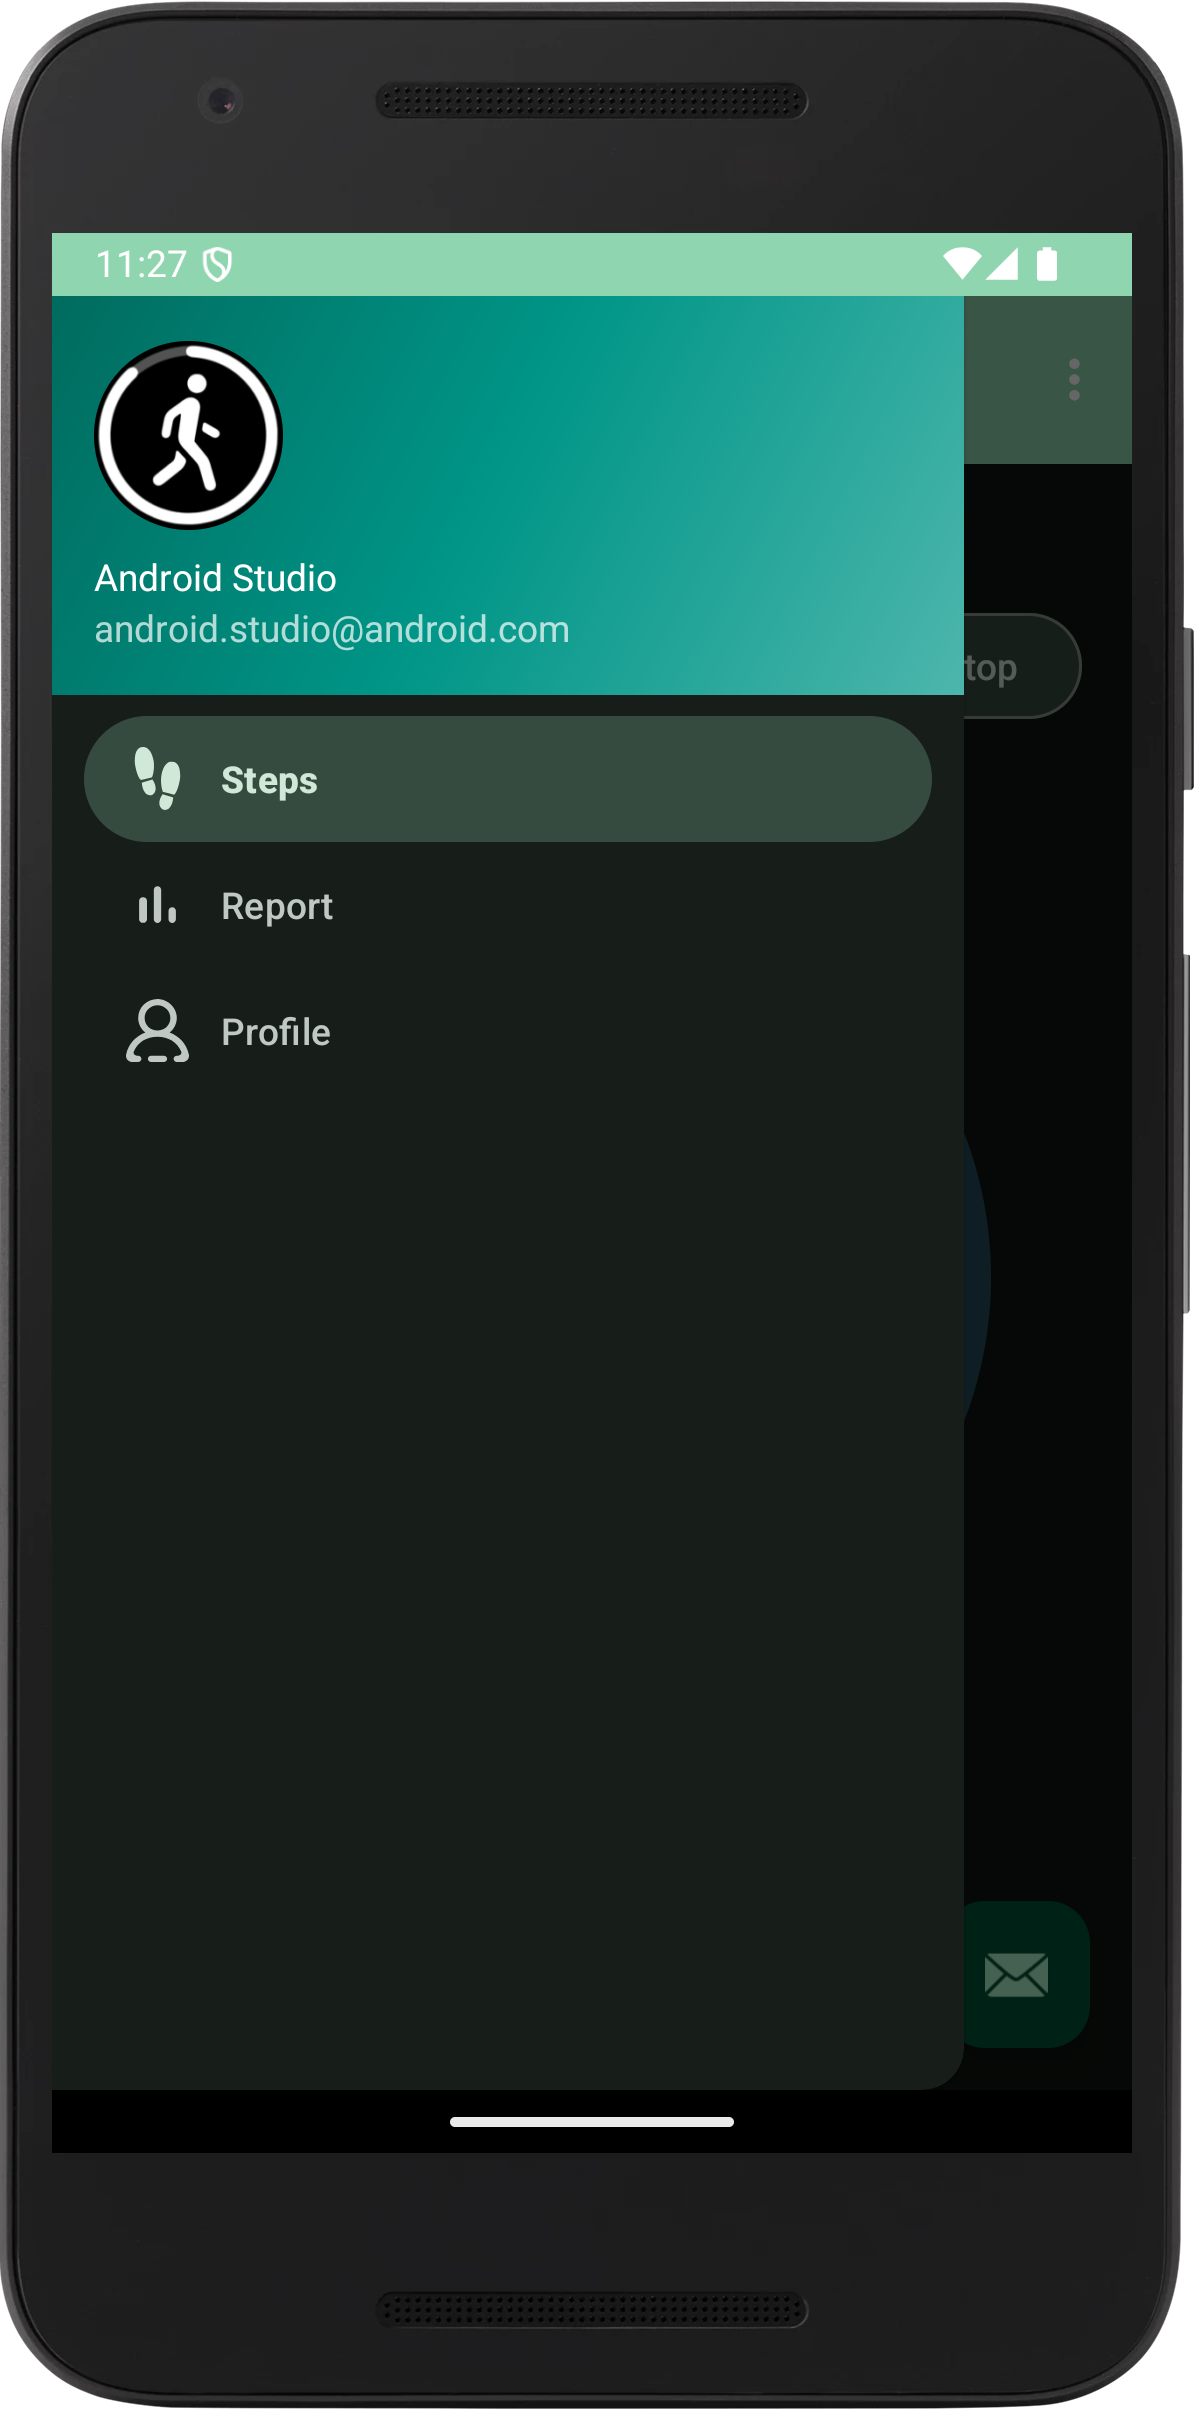
\includegraphics[width=0.15\textwidth]{res/img/darkMode3.png}
        \caption{App Screenshots in Dark Mode}
        \label{fig:ex2_2.4}
    \end{figure}

\newpage
\section{Exercise 3 – Step Counter}


\subsection{Android STEP\_DETECTOR}
First of all I modified the variable \texttt{accSensor} in the \texttt{StepsFragment} class to be of type:\\ \texttt{Sensor.TYPE\_STEP\_DETECTOR}. I could have easly have defined another variable but I wanted to make sure that all the counts were updted thanks to this sensor and not the previsouly used\\ \texttt{Sensor.TYP\_LINEAR\_ACCELERATION}.

\begin{verbatim}
    accSensor = sensorManager.getDefaultSensor(Sensor.TYPE_STEP_DETECTOR);
\end{verbatim}

Then I moved to the \texttt{StepCounterListener} class and mofied the \texttt{onSensorChanged} method to call the \texttt{countSteps} method. 

\lstinputlisting[
    firstline=101, 
    lastline=103, 
    firstnumber=101,
    caption=\texttt{\codepath/StepCounterListener.java}
]{\codepath/StepCounterListener.java}

\lstinputlisting[
    firstline=150, 
    lastline=156, 
    firstnumber=150,
    caption=\texttt{\codepath/StepCounterListener.java}
]{\codepath/StepCounterListener.java}
In this first part of the method I add the steps detected by the sensor to the step count variable, log the number of steps detected and save the current step count to the shared preferences.


\subsection{Update Circulat Progress Bar}
In the second part of method \texttt{countSteps} from the previous exercise I update the step count text view and the step count progress bar.

\lstinputlisting[
    firstline=150, 
    lastline=160, 
    firstnumber=150,
    caption=\texttt{\codepath/StepCounterListener.java}
]{\codepath/StepCounterListener.java}


\newpage

\subsection{Persistant Step Count}
In the last part of the \texttt{onCreate} method, I implemented functionality to load the number of steps from the database. This ensures that the step count persists after the user swtched to another fragment or even after the application is closed and reopened.

First, I retrieve the current timestamp and format it to extract the date. This is important because I want to load the step count corresponding to the current day. 

\lstinputlisting[
    firstline=99, 
    lastline=103, 
    firstnumber=99,
    caption=\texttt{\codepath/ui/steps/StepsFragment.java}
]{\codepath/ui/steps/StepsFragment.java}

Next, I use the \texttt{loadSingleRecord} method from the \texttt{StepAppOpenHelper} class to retrieve the number of steps for the current day. This method queries the database and returns the stored step count, which I then display on the \texttt{stepsTextView} and update the progress bar accordingly.

\lstinputlisting[
    firstline=105, 
    lastline=108, 
    firstnumber=105,
    caption=\texttt{\codepath/ui/steps/StepsFragment.java}
]{\codepath/ui/steps/StepsFragment.java}

\end{document}